
\section{Application options}
\subsection{General}
\index{secrets!general}

At the main menu click on \texttt{Options/Application}.
It will opens the window \texttt{Options/Application/Main/General}.

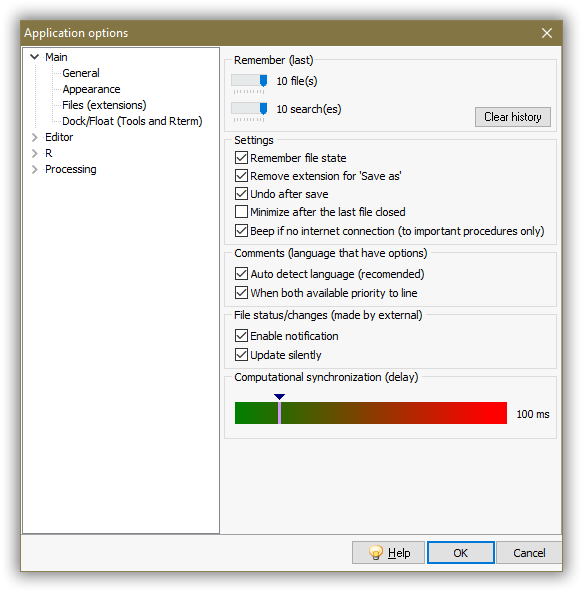
\includegraphics[scale=0.50]{./res/app_main_general.png}

One important options here is the \textit{Computational syncronization (delay)}.
Several processes are dependent on synchronization between applications
(\RR{}, converters, compilers). The optimal value of the delay is determined by the following characteristics:
user habits, hardware and software available.
The ideal value is unique to the various possible combinations of those three characteristics.
Try to reduce to the minimum value (50 ms) and test it: if something does not work, increase it gradually
and keep testing until getting to the optimal value. The default value (100 ms) may not be optimal for all users.


\subsection{Appearance}
\index{secrets!appearance}

At the \texttt{Option} window click on the tab \texttt{Main/Appearance}.
You can choose colors for each character's foreground (FG) and background (BG) color.
The color pallet will open and you can then choose the appropriate color.
For people working extensive periods of time in front of a computer monitor,
dark (or pale) colors with a low level of radiation are recommended for background,
obtaining a contrast with characters.

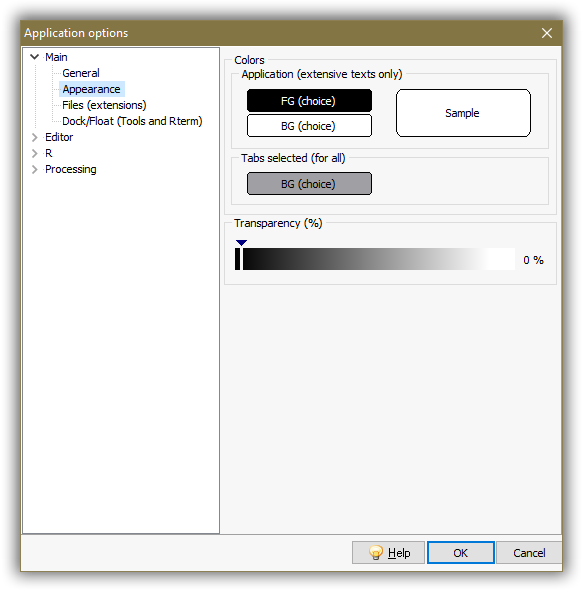
\includegraphics[scale=0.50]{./res/app_main_appearance.png}

\subsection{Dock}
\index{secrets!dock}

The dock contains a button called \texttt{Restore default}.
When clicked, every time you start Tinn-R the \texttt{Rterm} and \texttt{Tools} windows will be at the default position.
You usually do not want to mark it as you will lose your customization.
It is useful if any problem occurs with the resources (dock/hide and place).

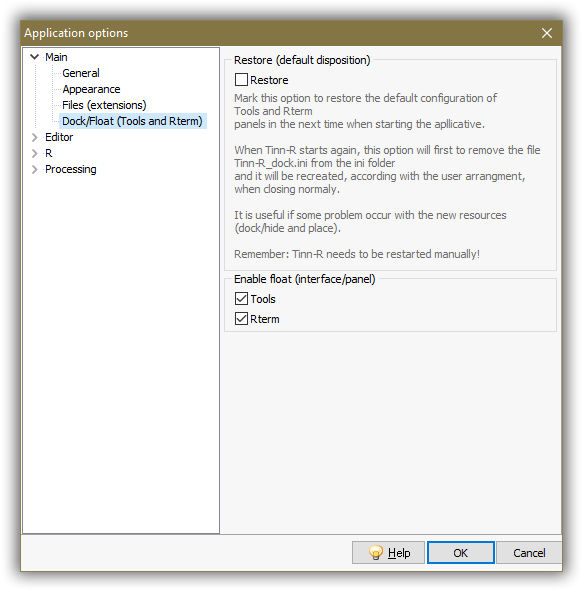
\includegraphics[scale=0.50]{./res/app_main_dock.png}


\subsection{Editor options}
\index{secrets!editor options}

The first window showing up is the \texttt{Display}. When first glancing at the editor window (where you type your scripts)
you may have noticed a thin vertical line which is located at exactly 80 characters (default) from the beginning of each line.
This is called the edge line. This line is very helpful to have a standard width for your texts,
mainly when you increase or reduce the font size (\texttt{CTRL + SHIFT + UP/DOWN})
as you increase the font the edge line keeps on moving to the right,
so that you can adapt the edge column to your preferred font size.

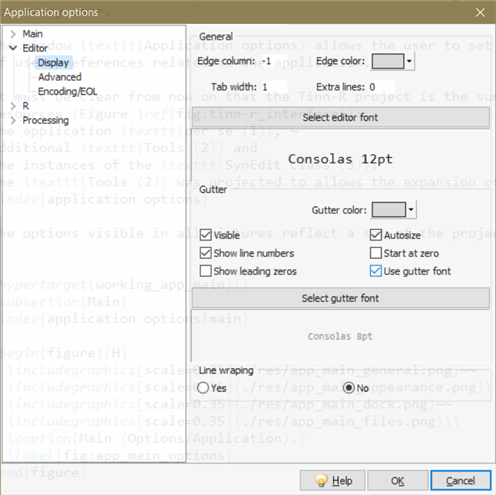
\includegraphics[scale=0.50]{./res/app_editor_display.png}

You may choose the font and the font size by clicking on font (\texttt{Consolas 11pt} is a nice option).
Gutter is the space at extreme left of the editor, out of the text window,
where you may number the lines of your script, just click at your choice.

For the other choice, \texttt{Advanced} options \textit{\href{\#working\_editor}{see Editor options}}.

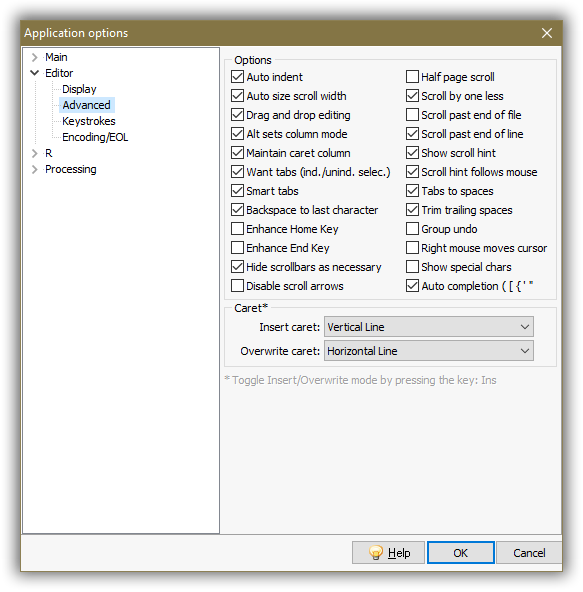
\includegraphics[scale=0.40]{./res/app_editor_advanced.png}~~

\subsection{R}
\index{secrets!R}

The first tab (\texttt{Path}) shows the paths to \textbf{Rterm.exe} or \textbf{Rgui.exe}.
You can also choose whether Tinn-R gets the latest installed version of \RR{} or the version you would like to use.
If you have Windows 7 64 bit choose that option located at the bottom of the window.

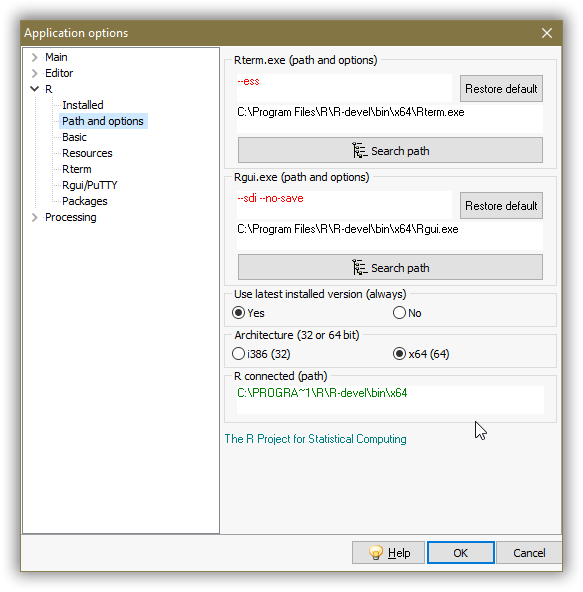
\includegraphics[scale=0.50]{./res/app_r_pathandoptions.png}

The next important tab is \texttt{Rterm}. The button \texttt{Trying to find errors (at the editor), yes}
means that errors in \RR{} syntax are searched within the editor to find where the error shows up the first
time within the script. You will usually have to keep on clicking the \texttt{F3} key until you find the error position.

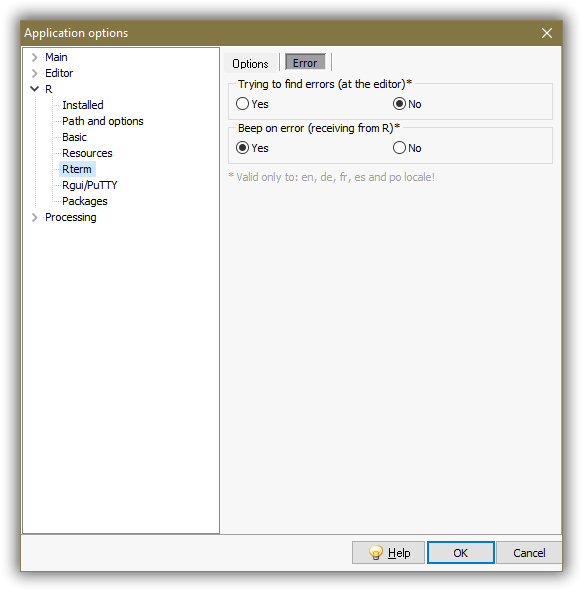
\includegraphics[scale=0.50]{./res/app_r_rterm_error.png}

\subsection{Processing}
\index{processing}
\index{processing!DVI}
\index{processing!PDF}

The tab \texttt{Processing} allows you to set preferences related to processing, namely text conversion and compilation.
For example, click on \texttt{Latex/PDF} at \texttt{Viewer} (we suggest to use Foxit Reader or Sumatra).
That, as it will be shown later, will enable you to compile \LaTeX ~texts and open them in \textit{.pdf} using Tinn-R.
Do not forget to install the Miktex on your computer. If you prefer DVI instead of PDF click on the DVI button.

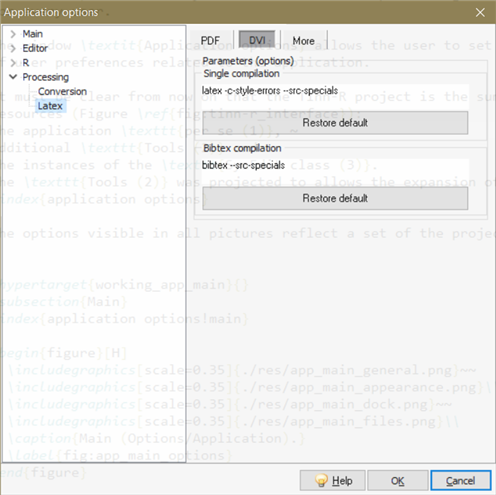
\includegraphics[scale=0.40]{./res/app_processing_latex_dvi.png}~~
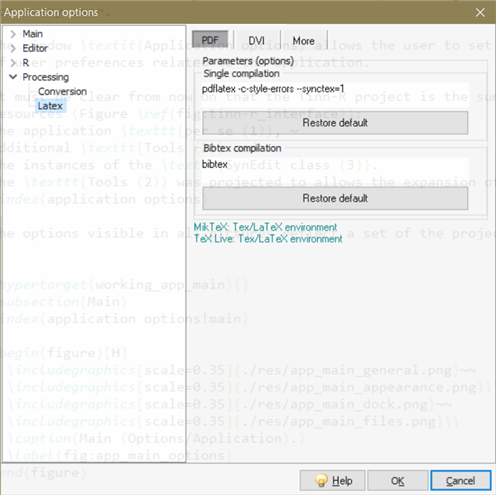
\includegraphics[scale=0.40]{./res/app_processing_latex_pdf.png}\\
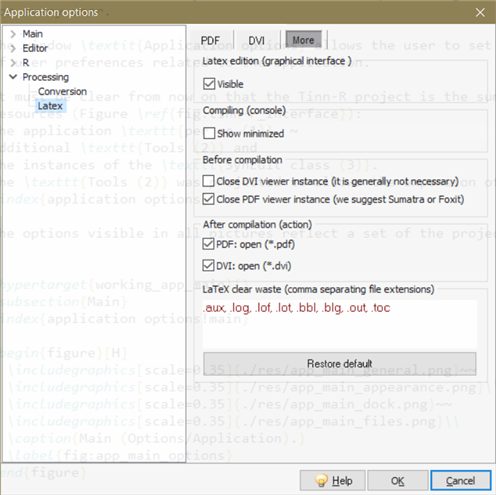
\includegraphics[scale=0.40]{./res/app_processing_latex_more.png}
